% This file is part of GUFI, which is part of MarFS, which is released
% under the BSD license.
%
%
% Copyright (c) 2017, Los Alamos National Security (LANS), LLC
% All rights reserved.
%
% Redistribution and use in source and binary forms, with or without modification,
% are permitted provided that the following conditions are met:
%
% 1. Redistributions of source code must retain the above copyright notice, this
% list of conditions and the following disclaimer.
%
% 2. Redistributions in binary form must reproduce the above copyright notice,
% this list of conditions and the following disclaimer in the documentation and/or
% other materials provided with the distribution.
%
% 3. Neither the name of the copyright holder nor the names of its contributors
% may be used to endorse or promote products derived from this software without
% specific prior written permission.
%
% THIS SOFTWARE IS PROVIDED BY THE COPYRIGHT HOLDERS AND CONTRIBUTORS "AS IS" AND
% ANY EXPRESS OR IMPLIED WARRANTIES, INCLUDING, BUT NOT LIMITED TO, THE IMPLIED
% WARRANTIES OF MERCHANTABILITY AND FITNESS FOR A PARTICULAR PURPOSE ARE DISCLAIMED.
% IN NO EVENT SHALL THE COPYRIGHT HOLDER OR CONTRIBUTORS BE LIABLE FOR ANY DIRECT,
% INDIRECT, INCIDENTAL, SPECIAL, EXEMPLARY, OR CONSEQUENTIAL DAMAGES (INCLUDING,
% BUT NOT LIMITED TO, PROCUREMENT OF SUBSTITUTE GOODS OR SERVICES; LOSS OF USE,
% DATA, OR PROFITS; OR BUSINESS INTERRUPTION) HOWEVER CAUSED AND ON ANY THEORY OF
% LIABILITY, WHETHER IN CONTRACT, STRICT LIABILITY, OR TORT (INCLUDING NEGLIGENCE
% OR OTHERWISE) ARISING IN ANY WAY OUT OF THE USE OF THIS SOFTWARE, EVEN IF
% ADVISED OF THE POSSIBILITY OF SUCH DAMAGE.
%
%
% From Los Alamos National Security, LLC:
% LA-CC-15-039
%
% Copyright (c) 2017, Los Alamos National Security, LLC All rights reserved.
% Copyright 2017. Los Alamos National Security, LLC. This software was produced
% under U.S. Government contract DE-AC52-06NA25396 for Los Alamos National
% Laboratory (LANL), which is operated by Los Alamos National Security, LLC for
% the U.S. Department of Energy. The U.S. Government has rights to use,
% reproduce, and distribute this software.  NEITHER THE GOVERNMENT NOR LOS
% ALAMOS NATIONAL SECURITY, LLC MAKES ANY WARRANTY, EXPRESS OR IMPLIED, OR
% ASSUMES ANY LIABILITY FOR THE USE OF THIS SOFTWARE.  If software is
% modified to produce derivative works, such modified software should be
% clearly marked, so as not to confuse it with the version available from
% LANL.
%
% THIS SOFTWARE IS PROVIDED BY LOS ALAMOS NATIONAL SECURITY, LLC AND CONTRIBUTORS
% "AS IS" AND ANY EXPRESS OR IMPLIED WARRANTIES, INCLUDING, BUT NOT LIMITED TO,
% THE IMPLIED WARRANTIES OF MERCHANTABILITY AND FITNESS FOR A PARTICULAR PURPOSE
% ARE DISCLAIMED. IN NO EVENT SHALL LOS ALAMOS NATIONAL SECURITY, LLC OR
% CONTRIBUTORS BE LIABLE FOR ANY DIRECT, INDIRECT, INCIDENTAL, SPECIAL,
% EXEMPLARY, OR CONSEQUENTIAL DAMAGES (INCLUDING, BUT NOT LIMITED TO, PROCUREMENT
% OF SUBSTITUTE GOODS OR SERVICES; LOSS OF USE, DATA, OR PROFITS; OR BUSINESS
% INTERRUPTION) HOWEVER CAUSED AND ON ANY THEORY OF LIABILITY, WHETHER IN
% CONTRACT, STRICT LIABILITY, OR TORT (INCLUDING NEGLIGENCE OR OTHERWISE) ARISING
% IN ANY WAY OUT OF THE USE OF THIS SOFTWARE, EVEN IF ADVISED OF THE POSSIBILITY
% OF SUCH DAMAGE.



\subsection{\gufiquery}

\gufiquery is the main tool used for accessing indicies. Arbitrary SQL
statements are passed into \gufiquery to run on the individual
databases, allowing for anything SQL can do to be done on the
databases in an index, including modifying the contents of each
database. To prevent accidental modifications from occuring, indicies
are opened in read-only mode by default.

Because \gufiquery uses SQL statements for database access, caller
will need to know about GUFI's database and table schemas. We expect
only ``advanced'' users such as administrators and developers to use
\gufiquery directly. Users who do not know how GUFI functions may call
\gufiquery, but might not be able to use it properly.

Just as indexing processes directories in parallel, the set of
queries passed into \gufiquery run on directories in parallel.

\subsubsection{Flags}

\begin{table} [H]
  \centering
  \begin{tabular*}{\linewidth}{l|p{0.5\linewidth}}
    Flag & Functionality \\
    \hline
    -h & help \\
    \hline
    -H & show assigned input values (debugging) \\
    \hline
    -E \textless SQL ent\textgreater & SQL for entries table \\
    \hline
    -S \textless SQL sum\textgreater & SQL for summary table \\
    \hline
    -T \textless SQL tsum\textgreater & SQL for tree-summary table \\
    \hline
    -a & AND/OR (SQL query combination) \\
    \hline
    -n \textless threads\textgreater & number of threads (default: 1) \\
    \hline
    -j & print the information in terse form \\
    \hline
    -o \textless out\_fname\textgreater & output file (one-per thread, with thread-id suffix) \\
    \hline
    -d \textless delim\textgreater & one char delimiter (default: \texttt{\textbackslash x1E}) \\
    \hline
    -O \textless out\_DB\textgreater & output DB \\
    \hline
    -I \textless SQL\_init\textgreater & SQL init \\
    \hline
    -F \textless SQL\_fin\textgreater & SQL cleanup \\
    \hline
    -y \textless min-level\textgreater & minimum level to descend to \\
    \hline
    -z \textless max-level\textgreater & maximum level to descend to \\
    \hline
    -J \textless SQL\_interm\textgreater & SQL for intermediate
    results (no default. ex.: \texttt{INSERT INTO \textless
      aggregate table name\textgreater \ SELECT * FROM \textless
      intermediate table name\textgreater}) \\
    \hline
    -K \textless create aggregate\textgreater & SQL to create the final aggregation table \\
    \hline
    -G \textless SQL\_aggregate\textgreater & SQL for aggregated
    results (no default. ex.: \texttt{SELECT * FROM
      \textless aggregate table name\textgreater}) \\
    \hline
    -m & Keep mtime and atime same on the database files \\
    \hline
    -B \textless buffer size\textgreater & size of each thread's output buffer in bytes \\
    \hline
    -w & open the database files in read-write mode instead of read only mode \\
    \hline
    -x & enable xattr processing \\
    \hline
    -k & file containing directory names to skip \\
    \hline
    -M \textless bytes\textgreater & target memory footprint \\
    \hline
  \end{tabular*}
  \caption{\label{tab:widgets} \gufiquery Flags and Arguments}
\end{table}

\subsubsection{Short Circuiting}
Although each table/view has a specific flag that they are associated
with, there is no need to use them with the flag. Queries are
free-form text, so there is no reliable way to limit their usage to a
particular flag.

The purpose of having separate flags was to allow for directory
processing to be short-circuited: if \texttt{-T} fails to return any
results, processing is stopped before running the \texttt{-S}
query. Similarly, if \texttt{-S} does not return any results, the
\texttt{-E} query is not run. This allows for threads to end the
processing of a directory early if it is determined early on that no
rows would be obtained from a later query. For example, if a query is
searching for files larger than 1MB, but the \texttt{-S} query found
that the range of file sizes is 1KB to 5KB, there is no need to run
the \texttt{-E} query to get rows, since no rows will match in any
case.

To turn off short circuiting and always run all queries for each
directory, pass the \texttt{-a} flag to \gufiquery.

\subsubsection{Extended Attributes}
When querying for xattrs, pass \texttt{-x} to \gufiquery to build the
\xattrs view for querying. This view is a SQL union of rolled in
xattrs and any external databases that successfully
attaches. Attaching the database files checks the permissions of the
xattrs. \texttt{UNION} removes duplicate entries that showed up in
multiple external databases, leaving a unique set of xattrs accessible
by the caller.

The \xentries, \xpentries, \xsummary views are convenience views
generated so that users do not have to perform joins themselves. They
are \entries, \pentries, and \summary enhanced with the
\texttt{xattr\_name} and \texttt{xattr\_value} columns. Like the
\xattrs view, these views are also dropped at the end of directory
processing.

Note that entries with multiple extended attributes will return
multiple times in this view.

\subsubsection{Aggregation}
There are cases where independent per-thread results are not
desirable, such as when sorting or summing, where the results from
querying the index must be aggregated for final processing.

In order to handle these situations, the \texttt{-I} flag should be
used to create per-thread intermediate tables that are written to by
\texttt{-S} and \texttt{-E}. The intermediate table results will then
be aggregated using \texttt{-J} into the final table created by
\texttt{-K}. The rows stored in the final table are processed one last
time as a whole, rather than as results from independent threads,
using \texttt{-G}.

\subsubsection{Per-Thread Output Files}
The \texttt{-o} flag causes results to be outputted to text
files. When outputting in parallel, per-thread output files are
created with the thread id appended to the filename provided with the
flag. When aggregating, the aggregate results are written to the
filename specified by \texttt{-o} with no filename modifications.

\subsubsection{Per-Thread Output Database Files}
The \texttt{-O} flag allows for results to be written to SQLite
database files instead of text files. The resulting filenames follow
the same creation rules as \texttt{-o}. However, the queries passed
into \gufiquery need modifications. When writing in parallel,
\texttt{-I} is needed to create the table for each per-thread output
database. \texttt{-S} and \texttt{-E} should be modified to write to
the per-thread tables in the same way as writing to the intermediate
tables when aggregating. When writing aggregate results, \texttt{-G}
is not needed, as \texttt{-J} already wrote the results into the
aggregate table. However, \texttt{-G} may still be provided to get
results during the \gufiquery in addition to queries on the results
database file later on.

Output database files may be passed to the \querydbs executable for
further processing.

\subsubsection{Example Calls}

\noindent Parallel Results:
\\\\
\indent \gufiquery \texttt{-S "SELECT * FROM summary"
  ~/directory\_of\_root\_index}
\\\\
\indent \gufiquery \texttt{-E "SELECT * FROM pentries"
  ~/directory\_of\_root\_index}
\\\\
\noindent Aggregate Results:
\\\\
\indent \gufiquery \texttt{\textbackslash} \\
\indent \texttt{-I "CREATE TABLE intermediate(name TEXT, size INT64);" \textbackslash} \\
\indent \texttt{-E "INSERT INTO intermediate SELECT name, size FROM pentries;" \textbackslash} \\
\indent \texttt{-K "CREATE TABLE aggregate(name TEXT, size INT64);" \textbackslash} \\
\indent \texttt{-J "INSERT INSERT aggregate SELECT * FROM intermediate;" \textbackslash} \\
\indent \texttt{-G "SELECT * FROM aggregate ORDER BY size DESC;"} \\

\subsubsection{Visualizing the Workflow}
\begin{figure} [H]
  \centering
  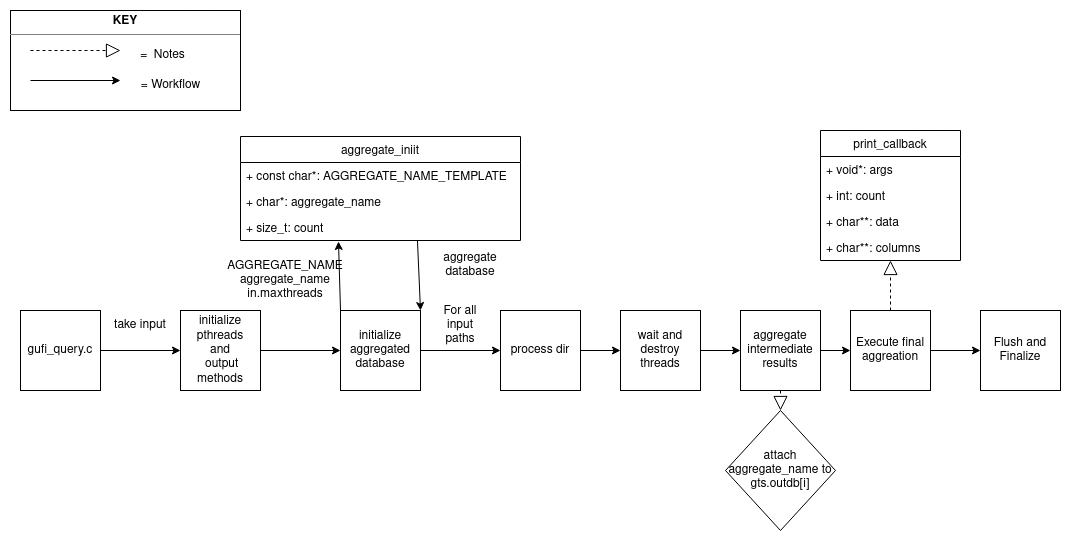
\includegraphics[width=\textwidth]{images/gufi_query_main.png}
  \caption{Workflow of \gufiquery}
\end{figure}

\subsubsection{\processdir}
The core of \gufiquery is the \processdir function. This is where the
-T, -S, and -E flags are processed. Multiple instances of this
function are run in parallel via the thread pool in order to quickly
traverse and process an index.

\begin{figure} [H]
  \centering
  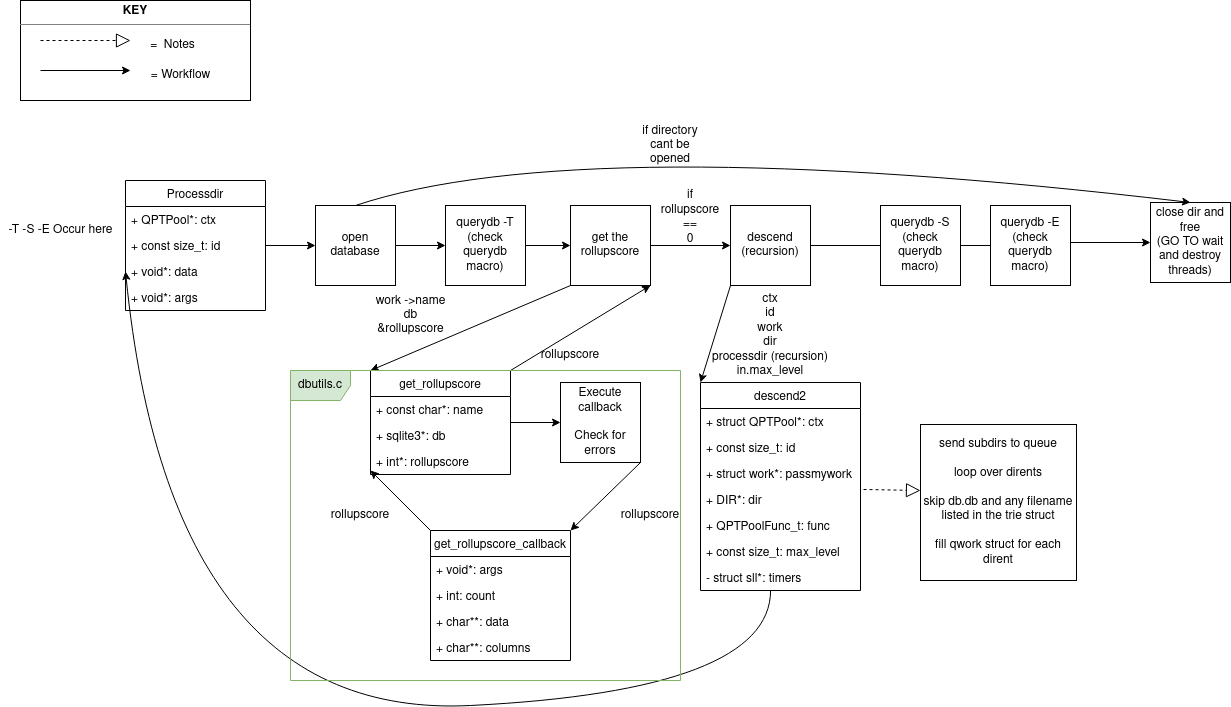
\includegraphics[width=\textwidth]{images/gufi_query_processdir.png}
  \caption{Workflow of \processdir}
\end{figure}

\subsubsection{\querydb macro}
\querydb is the macro used to execute SQL statements and handle errors.

\begin{figure} [H]
  \centering
  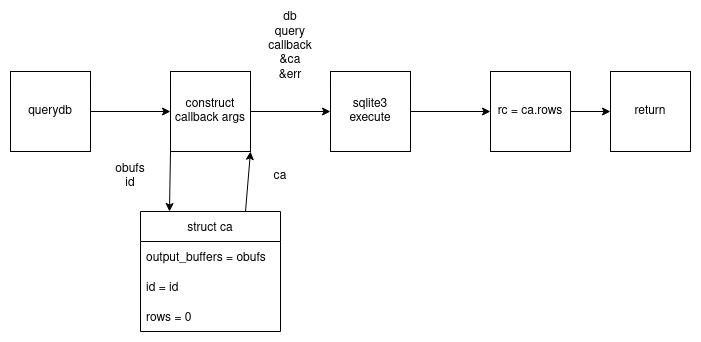
\includegraphics[width=\textwidth]{images/querydb_macro.png}
  \caption{\querydb macro workflow}
\end{figure}
